% A chapter named 'Your first document' is created
\chapter{Componenten} \label{cha:componenten}


\section{Hoofdscherm} \label{sec:hoofdscherm}
\begin{figure}[h]
  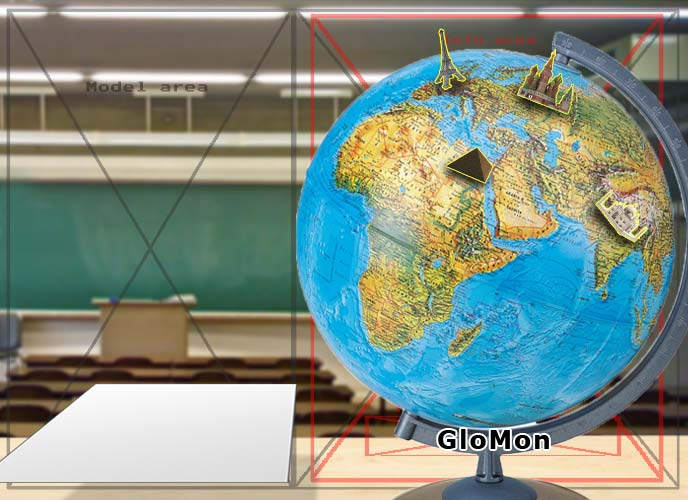
\includegraphics[width=130mm]{figs/components1a.jpg}
  \caption{Componenten hoofdscherm \textit{(27-April-2014)}}
  \label{fig:components1}
\end{figure}

Het hoofdscherm is een reflectie van het camerabeeld dat wordt opgenomen. Het achterliggende transparante wireframe is hier slechts te zien ter verduidelijking, bij release van de applicatie zal deze niet  zichtbaar zijn. De applicatie is alleen bruikbaar is bij een specifieke wereldbol die is voorzien van speciale markering en dient om de positie van de 3D modellen op de bol aan te sturen. Links van het scherm is een kaart te zien, deze kaart bevat ook speciale markeringen die gebruikt zullen worden om het 3D model weer te geven.

\newpage
\section{Infoscherm} \label{sec:infoscherm}
\begin{figure}[h]
  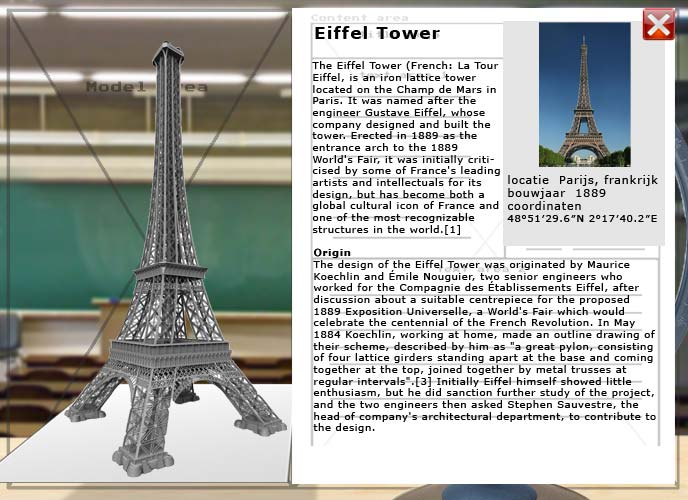
\includegraphics[width=130mm]{figs/components2a.jpg}
  \caption{Componenten infoscherm \textit{(27-April-2014)}}
  \label{fig:components2}
\end{figure}
Zodra de gebruiker een monument selecteerd, zal er een info paneel openen met informatie over het monument. Ook zal op de kaart een 3D model worden weergegeven met het geselecteerde model. De gebruiker kan de kaart draaien om het model vanaf verschillende hoeken te bekijken.

\newpage
\section{Digitale componenten} \label{sec:digicomponents}
\begin{figure}[h]
  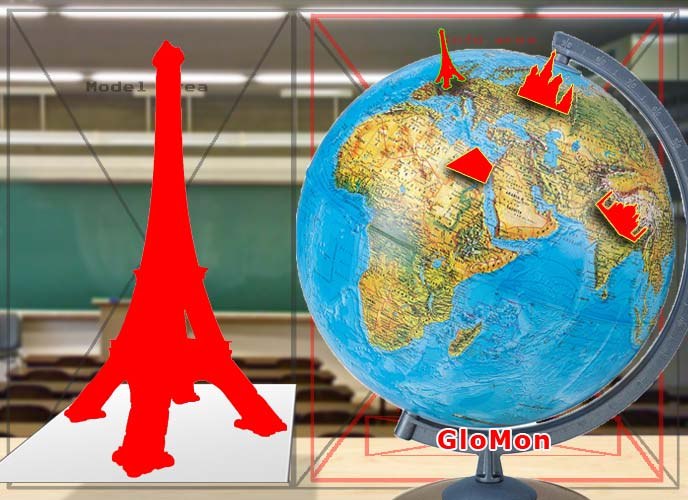
\includegraphics[width=130mm]{figs/components4a.jpg}
  \caption{Digitale componenten (rood) \textit{(27-April-2014)}}
  \label{fig:digitals}
\end{figure}

In het rood zijn alle elementen weergegeven die digitaal zullen worden weergegeven. Afhankelijk van de positie van de wereldbol zullen er 3D modellen worden weergegeven op de reflectie van de wereldbol op het scherm. Deze modellen draaien volledig mee met de assen van de wereldbol. Een geselecteerd model wordt gehighlight zodat het voor de gebruiker duidelijk is dat er iets is geselecteerd (In \cref{fig:digitals} heeft de Eiffel toren op de bol bijvoorbeeld een groene rand). Na selectie wordt er ook een 3D model op de fysieke kaart weergegeven.